\chapter{Structural and accidental phonotatic gaps}
\label{gaps}

Early work in generative phonology notes that neutralizing, surface-true phonological alternations impose constraints both on surface forms and underlying representations (\citealp[283]{Anderson1974}, \citealp[382]{SPE}, \citealp[205f.]{Dell1973}, \citealp[22f.]{SPR}, \citealp{Kisseberth1970b}, \citealp{Kenstowicz1977}: chap.~3, \citealp[28f.]{Stampe1973}, \citealp[410f.]{Stanley1967}). 

Two domains are essential to defining 

Despite isolated claims to the contrary (e.g., \citealp[297]{Hale1965}; \citealp[212f.]{Postal1968}), 

\begin{quote}
It would be a result of the greatest interest if it were to turn out that every intramorphemic regularity was necessarily reflected in an alternation, and thus in a rule; but this position cannot seriously be maintained. \citep[283]{Anderson1974}
\end{quote}

\section{English syllable contact clusters}

English admits a variety of word-medial consonant clusters spanning syllable boundaries; these are known as \emph{syllable contact clusters} or \emph{interludes}. \citeauthor{Pierrehumbert1994} presents the following as a null hypothesis for which clusters are admissible in some language, echoing a similar proposal by \citet{Haugen1956}.

\begin{quote}
\ldots{}in the absence of additional provisos, any concatenation of a well-formed coda and a well-formed onset is predicted to be possible medially in a word. \citep[][168]{Pierrehumbert1994}
\end{quote}

Many phonotactic generalization can be thought of as restrictions on the inventory of different prosodic constituents defining what is, e.g., a ``well-formed onset''. Since few linguists posit the interlude as a prosodic constituent \citep[though cf.][]{Steriade1999}, further constraints on syllable contact clusters, however, are combinatoric.

\section{Evaluation}
\label{4evaluation}

\subsection{Method}

\subsubsection{Materials and procedure}

Following \citet[ chap.~8]{Duanmu2009} and \citet[ chap.~3]{Hammond1999a}, 
a wordlist was produced using the English portion of the CELEX database \citep{CELEX}. Any words which were coded as borrowings were excluded, as were all words not coded as ``monomorphemic''. The use of this stringent criterion eliminates many of the exceptions noted by \citeauthor{Duanmu2009} or \citeauthor{Hammond1999a} in their studies. For instance, many of the exceptions to \textsc{Obstruent Voice Assimilation} (see \S? below) noted by \citet[74]{Hammond1999a} are coded either as loanwords (e.g., \emph{vodka}, \emph{smorgasbord}) or as complex words (e.g., \emph{jurisdiction}, \emph{madcap} \emph{tadpole}, \emph{scapegoat}, \emph{magpie}). 

Unlike prior studies, ``neo-classical compounds'', words which appear to consist of a Latinate prefix and a bound stem (e.g., \emph{inspect}, \emph{excrete}) are also excluded from this wordlist. This is done in response to converging evidence that English speakers regard such words as complex. 

The baroque treatment of Latinate forms in \emph{The sound pattern of English} (\citealp{SPE}, henceforth \emph{SPE}) assumes a prefix/bound stem decomposition to simplify various morphophonological generalizations. 

In a similar vein, \citet[11f.]{Aronoff1976} observes that Latinate forms which share the same bound stem also share irregular allomorphs of that stem under derivation, which is presented as evidence of prefix/bound stem decomposition.

\begin{example}[Bound stem-specific allomorphy]
\begin{tabular}{l l l l l l}
a. & {adhere}   & {adhesion}   \\
   & {cohere}   & {cohesion}   \\
b. & {conceive} & {conception} \\
   & {perceive} & {perception} \\
\end{tabular}
\end{example}

This assumption has long been made to simplify phonological \citep{SPE}, allomorphic \citep[11f.]{Aronoff1976}, and syntactic \citep{Harley2009} generalizations. 

Results from lexical decision experiments also suggest that neoclassical compounds are complex. \citet{Taft1986} and \citet{Taft1975,Taft1976} find that nonce words like \emph{*re-sert}, which appear to be composed of a prefix and a bound stem, take longer to reject that non-words which lack apparent morphological structure such as *\emph{refant}). Bound stems also show frequency effects which are independent of their whole word frequency \citep{Taft1979,Taft2006}. Finally, \citet{Emmorey1989} and \citet{Forster2000} report facilitative priming between pairs like \emph{permit}-\emph{submit}, an effect suggestive of a shared morphological identity.  

There is also a syntactic interaction between Latinate prefixes on verbs and the makeup of the verbal complement. \citet{Harley2009} observes that Latinate verbs do not generally participate in ditransitive, verb participle, or adjectival resultative constructions, all acceptable with similar Anglo-Saxon verbs \citep[see also][]{Gropen1989,Coppock2008}. \citeauthor{Harley2009} proposes that the Latinate prefix is introduced in a low small clause, the same position as the theme, participle, and result adjectival in the Anglo-Saxon examples.

\begin{example}[Latinate verbs and small clauses] 
\label{harley}
\begin{tabular}{l l l l@{} l}
a. & {show him the painting} & \alt{} & * & {exhibit him the painting} \\
b. & {drink himself stupid}  & \alt{} & * & {imbibe himself stupid}    \\
c. & {show it off}           & \alt{} & * & {exhibit it off}           \\
\end{tabular}
\end{example}

This filtering results in a list of 6,619 simplex words. The CELEX transcriptions of these words were then syllabified and phonologized using a technique described in Appendix \ref{syllabification}. This produces 23 unique medial codas and 40 unique medial onsets. Of the 920 ($= 21 \times 40$) medial clusters that would result from free combination, 174 (19\%) are attested. The full set of clusters and their frequencies are reproduced in Appendix \ref{clusters}. 

\subsection{Results}

\subsubsection{Static constraints}

There is no statistical support for any of the three static constraints proposed by \citeauthor{Pierrehumbert1994}. 
%However, it is premature to conclude that no static constraint exists. It is possible that an explicit model of ``constraint discovery'', could identify reliable static constraints,

\subsubsection{Derived constraints}

\paragraph{Obstruent voice assimilation}

Voice assimilation alternations are evidenced by the non-syllabic allomorphs of the regular past (e.g., \emph{nap}[t] $\sim$ \emph{nab}[d]) and noun plural (e.g., \emph{lap}[s] $\sim$ \emph{lab}[z]), which take the voicing specification of a preceding obstruent.\footnote{Underlying /-d, -z/ are assumed here (e.g., \citealt{Anderson1973a}, \citealt[284f.]{Bakovic2005b}, \citealt{Basboll1972}, \citealt[210]{SPE}, \citealt[282]{Hockett1958}, \citealt[102]{Pinker1988}, \citealt{Shibatani1972}); alternative analyses are put forth by \citet[210f.]{LANGUAGE}, \citet[135]{Borowsky1986}, \citet{Hoard1971}, \citet{Kiparsky1985}, \citet{Lightner1970}, \citet{Luelsdorff1969}, \citet{Miner1975}, \citet[426]{Nida1948}, and \citet{Zwicky1975}.}

\begin{example}[\textsc{Obstruent Voice Assimilation}]
\label{ovarule}
$\begin{bmatrix} -\textsc{Son} \end{bmatrix}~\goesto~\begin{bmatrix} =\textsc{Voi} \end{bmatrix}~/~\gap~\begin{bmatrix} =\textsc{Voi} \\ -\textsc{Son} \end{bmatrix}$
\end{example}

\noindent
\citet{Pierrehumbert1994} does not discuss a constraint against adjacent obstruents disagreeing in voice. As shown in Table \ref{ovatab} however, the vast majority of medial obstruents clusters in simplex words are either uniformly voiced, as in \emph{hu}[z.b]\emph{and}, or uniformly voiceless, as in or \emph{rha}[p.s]\emph{osdy}. Hetero-voiced clusters, like those in \emph{a}[b.s]\emph{inth} and \emph{a}[s.b]\emph{estos} are rare in comparison.

\begin{table}
\centering
\begin{tabular}{l rrrr}
\toprule
           & attested & unattested & saturation & $p$-value \\
\midrule
conforming & 35       & 329        & 10\%       & \multirow{2}{*}{0.002} \\
violating  & 11       & 305        &  3\%       \\
\bottomrule
\end{tabular}
\caption{FIXME}
\label{ovatab}
\end{table}

\paragraph{Nasal place assimilation}
\label{npa}

\textsc{Nasal Place Assimilation} (\emph{SPE}:85) accounts for [n $\sim$ ŋ] allophony as well as 

is responsible for the allomorphs of the \emph{im-}/\emph{in-} prefix, determined by the place of the following consonant (though there are additional complexities; see \citealt{Borowsky1986}:?, \citealt{Halle1985a}, \citealt{Jensen2000}).

\begin{example}[\emph{im-}/\emph{in-} allomorphy]
\label{nparule}
\begin{tabular}{l l l l l l l}
a. & {polite}   & {i}[m.p]{olite}   & & {balance} & {i}[m.b]{alance} \\
b. & {tangible} & {i}[n.t]{angible} & & {decent}  & {i}[n.d]{ecent}  \\
\end{tabular}
\end{example}

\begin{example}[\textsc{Nasal Place Assimilation}]
$\begin{bmatrix} $+$\textsc{Nas} \end{bmatrix}~\goesto~\begin{bmatrix} =\textsc{Lab} \\ =\textsc{Cor} \\ =\textsc{Dor} \end{bmatrix}~/~\gap{}~\begin{bmatrix} =\textsc{Lab} \\ =\textsc{Cor} \\ =\textsc{Dor} \\ -\textsc{Son} \end{bmatrix}$
\end{example}

\begin{table}
\centering
\begin{tabular}{l rrrr}
\toprule
           & attested & unattested & saturation & $p$-value \\
\midrule
conforming & 31       & 2          & 94\%       & \multirow{2}{*}{3.37\e{-07}} \\
violating  & 11       & 22         & 33\%       \\
\bottomrule
\end{tabular}
\caption{FIXME}
\label{npatab}
\end{table}

\paragraph{Degemination}

The final alternation found in English medial clusters is the simplification of geminates characteristic of ``level I'' morphology. Verb roots ending in /d/ which select the irregular /-t/ past tense suffix exhibit degemination (e.g., \emph{bend}/\emph{ben}[t], \emph{build}/\emph{buil}[t]). 

A final alternation targeting English syllable contact clusters is the simplification of geminates certain affixes. 

The deadjectival suffix \emph{-ly} does not result in a geminate \emph{l} when it attaches to 

krarely produces a geminate when it attaches to /l/-final roots (e.g., \emph{norma}[l]\emph{y}, cf. \emph{calm}[l]\emph{y}). 


More complicated cases of \textsc{Degemination} can be found in Latinate prefix allomorphy (\emph{SPE}:148; \citealp[102]{Borowsky1986}).


\begin{example}[\textsc{Degemination}]
$\begin{bmatrix} =\textsc{Lab} \\ =\textsc{Cor} \\ =\textsc{Dor} \\ =\textsc{Son} \\ \ldots{} \end{bmatrix}~\goesto~\emptyset~\big /~\gap~\begin{bmatrix} =\textsc{Lab} \\ =\textsc{Cor} \\ =\textsc{Dor} \\ =\textsc{Son} \\ \ldots{} \end{bmatrix}$
\end{example}

\begin{table}
\centering
\begin{tabular}{l rrrr}
\toprule
           & attested & unattested & saturation & $p$-value \\
\midrule
conforming & 173      & 643        & 21\%       & \multirow{2}{*}{1.2\e{-10}} \\
violating  & 0        & 104        & 0\%        \\
\bottomrule
\end{tabular}
\caption{FIXME}
\label{degemtab}
\end{table}

\subsubsection{Computational models}

A soft-margin support vector machine \citep{Cortes1995} with a linear kerne
l is used to convert from the per-cluster scores to attestation predictions
, by finding a single cutoff which optimally separates attested and unattes
ted clusters according to their model scores. This is in no way intended to
 be a cognitively plausible model for learning phonotactics; it simply repr
esents an upper bound on the performance of these models. The results for a
ll four models are summarized in Table \ref{cmresults}.

\begin{table} 
\centering
\begin{tabular}{l | rrrr}
\toprule
                    & accuracy & precision & recall & $F_1$ \\
\midrule
Baseline            & 0.812    & 0.812     & 1.000  & 0.896 \\
\citet{Hayes2008a}  & 0.835    & 0.942     & 0.854  & 0.896 \\
Expected frequency  & 0.836    & 0.845     & 0.984  & 0.909 \\
Derived constraints & 0.838    & 0.840     & 0.997  & 0.912 \\
DC and EF           & 0.861    & 0.868     & 0.988  & 0.924 \\
\bottomrule
\end{tabular}
\caption{FIXME}
\label{cmresults}
\end{table}

\subsection{Discussion}

\subsubsection{The probability of accidental gaps}

\begin{unlabeledexample}
$\displaystyle \hat{p}_0 = \frac{n_1}{N}$
\end{unlabeledexample}

%67 types occur once
%67 / 977
%7\% 

\subsubsection{Simulating medial clusters}

\begin{example}[Simulation procedure]
\begin{tabular}{l l}
a. & Sample a medial coda according to the observed probabilities  \\
b. & Sample a medial onset according to the observed probabilities \\
c. & Apply all matching \emph{SPE} rules to cluster formed by their concatenation \\
\end{tabular}
\end{example}

\begin{figure}
\centering
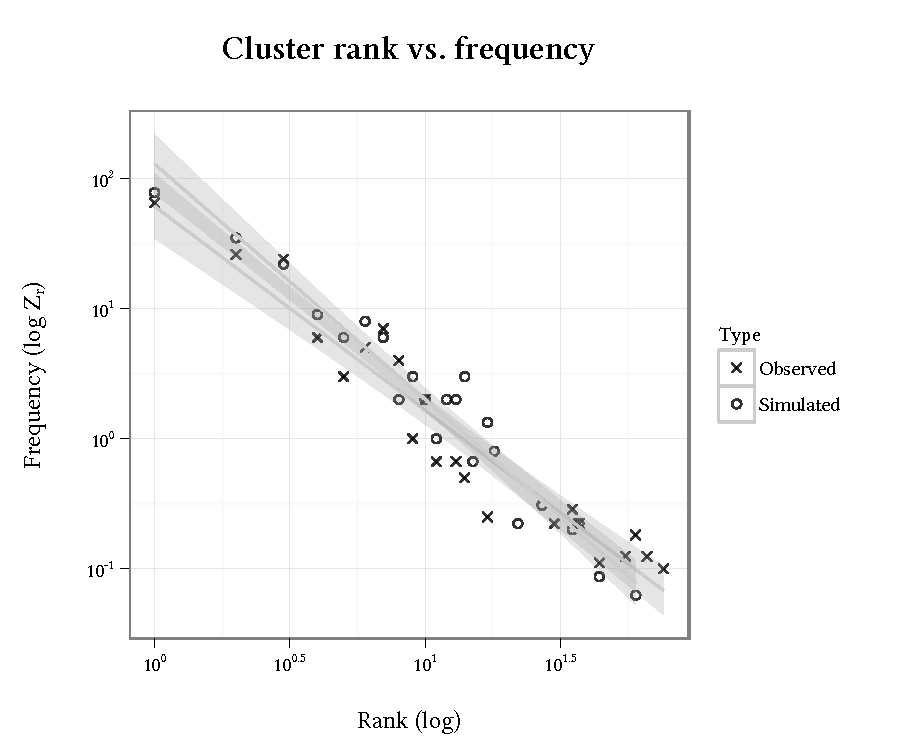
\includegraphics{sim.pdf}
\caption{A simulated cluster inventory, generated by random sampling and applying phonological neutralizations closely matches the observed cluster frequencies (represented by the smoothing line). Both simulated and observed frequencies have been smoothed using the $Z_r$ transform.}
\label{sim}
\end{figure}

real ($\alpha = -1.65$, $R^2 = 0.940$)
fake ($\alpha = -1.58$, $R^2 = 0.945$)
fitt ($R^2 = 0.712$, $p = 4.5$\e{-05})

\section{Conclusions}

%however, the \emph{communis opinio} still is that that not all phonotactics---that is, language-specific sound sequence co-occurrence restrictions---can be derived in this fashion, and phonotactic knowledge is independent of the phonology.
%
%%FIXME
%% \citet[255]{Anderson1974}, discussing this fact, writes that \citeauthor{Haugen} ``gives an argument that shows the necessity of including syllables as units in underlying representations''.
%
%%FIXME
%(for dissenting views, see \citealt{Blevins2003} and \citealt{Steriade1999})
%
%Linguists have long recognized underlying representations as privileged domains for stating phonotactic generalizations (e.g., \citealt{Bloomfield1930,Jakobson1932,Pike1947b}). 
%
%More recently, a similar role for the syllable has been recognized 
%(e.g., \citet{Haugen1956}, \citet{Hooper1973}, \citealt{Kahn1976})
%
%
%\begin{quote}
%It would be a result of the greatest interest if it were to turn out that every intramorphemic regularity was necessarily reflected in an alternation, and thus in a rule; but this position cannot seriously be maintained. \citep[283]{Anderson1974}
%\end{quote}
%
%
%\begin{quote}
%It would be a result of the greatest interest if it were to turn out that every intramorphemic regularity was necessarily reflected in an alternation, and thus in a rule; but this position cannot seriously be maintained. \citep[283]{Anderson1974}
%\end{quote}
%
%English word-medial consonant clusters have been used, by \citet{Pierrehumbert1994} and others, to argue for the necessity of an independent phonotactics module and illustrate proposals for its architecture. This chapter argues, however, that the only structural constraints on the concatenation of codas and onsets to form word-medial clusters are derivative of well-documented phonological alternations in English.
%
%\section{Background}
%
%English admits a variety of word-medial consonant clusters spanning syllable boundaries, known as \emph{syllable contact clusters} or \emph{interludes}. These clusters can be as short as two consonants (e.g., \emph{a}[n.t]\emph{ics}; singleton intervocalic consonants are ignored here) or as long as four (e.g., \emph{mi}[n.str]\emph{el}). \citeauthor{Pierrehumbert1994} presents the following as a null hypothesis for which clusters are admissible in any given language \citep[cf.][]{Haugen1956}.
%
%\begin{quote}
%\ldots{}in the absence of additional provisos, any concatenation of a well-formed coda and a well-formed onset is predicted to be possible medially in a word. \citep[][168]{Pierrehumbert1994}
%\end{quote}
%
%This chapter is concerned with the nature of these ``provisos'' as reflected by which of the ``possible'' clusters, so defined, are attested. While many phonotactic generalizations can be thought of as inventory restrictions imposed by prosodic constituents, additional filters on the set of possible clusters are essentially combinatoric in nature and thus distinct, there is no prosodic constituent consisting of the coda of one consonant-final syllable and the onset of a following consonant-initial syllable \citep[though see][]{Steriade1999}.
%
%\section{Evaluation}
%
%\citeauthor{Pierrehumbert1994} argues that the inventory of clusters in English shows the effect of a small number of static phonotactic constraints. The remainder of this chapter provides an exhaustive quantitative evaluation of this hypothesis. The most important constraints on medial clusters are those derived from phonological rules which apply across syllable boundaries; there is no remaining role for static constraints. The sparse nature of the lexicon plays a secondary role, giving rise to apparent phonotactic gaps even in the absence of static phonotactic constraints.
%
%\subsection{Corpus construction}
%
%A list of medial clusters is gathered by applying a number of filters and transformations to an English lexical database. The resulting list of clusters is reproduced in Appendix \ref{appendixC} and in electronic form at the author's website.
%
%\subsubsection{Simplex words}
%
%An analysis of lexical constraints requires a corpus of lexical representations. So as to remain agnostic about particulars of morphological theory, the goal here is to identify words which bear no overt inflection, and which do not admit any plausible further decomposition, henceforth ``simplex words''. For the structuralists, a procedure for parsing words into morphs, just the thing for locating simplex words, held the status of ``philosopher's stone'', a sort of near-mythical objective of the endeavor, but actual attempts to develop such a procedure \citep[e.g.,][]{Harris1955,Nida1948} are now recognized as anything but theory-neutral. Yet, there is no alternative to adopting some computational procedure or human-coded database as the ``gold standard'' for a study of this type. \citet{Pierrehumbert1994} analyzes a list of entries in the Collins English dictionary by hand, using her intuitions to filter out ``complex'' words as well as those which are not ``reasonably familiar''. Unfortunately, the resulting list was neither published nor circulated, and the possibility of replicating \citeauthor{Pierrehumbert1994}'s' sensations of morphological complexity is remote. Following prior studies of syllable contact clusters by \citet[ chapter 3]{Hammond1999a} and \citet[ chapter 8]{Duanmu2009}, a list of simplex words was derived from the ``lemmas'' (that is, uninflected forms) in the English portion of CELEX \citep{CELEX}, a database of morphological, phonological, and syntactic annotations based on the COBUILD corpus, a resource that was also used to construct the Collins English dictionary employed by \citeauthor{Pierrehumbert1994}.
%
%Two further filters were applied to this list. First, any lemma coded as an unassimilated loanword is excluded. Secondly, all lemmas that have a ``morphological status'' other than ``monomorpheme'' are excluded. This is crucial because CELEX makes no guarantee that lemmas are simplex; indeed, many lemmas are products of derivation (e.g., \emph{abusive}, from \emph{abuse}). These stringent criteria have a profound effect on the makeup of the data. For instance, nearly all exceptions to \textsc{Obstruent Voice Assimilation} (see \S\ref{ova} below) cited by \citet[74]{Hammond1999a} are excluded as unassimilated loanwords (e.g., \emph{vodka}, \emph{smorgasbord}) or as morphologically complex (e.g., \emph{jurisdiction}, \emph{madcap}, \emph{tadpole}, \emph{scapegoat}, \emph{magpie}). 
%
%``Neo-classical compounds'', words that appear to consist of a Latinate prefix and a bound stem, like \emph{inspect} or \emph{excrete}, have an ambiguous and long-debated morphological status. \citeauthor{Pierrehumbert1994} attempts to distinguish between words like \emph{complete}, \emph{extreme}, \emph{inspect}, \emph{obtuse}, which she assumes to be simplex, and \emph{excrete} and \emph{transparent}, which she considers complex. However, CELEX codes these words as complex and they are thus excluded. This is consistent with converging evidence that speakers decompose these Latinate forms. 

%Decomposition is also supported by lexical decision results. Among nonce words, those that can be exhaustively decomposed into prefix and bound stem, like *\emph{de}-\emph{juvenate}, are processed slower that contain a licit morph but cannot be exhaustively decomposed, like *\emph{de-pertoire}, and these in turn are processed slower than those which admit no such decomposition \citep{Taft1975}.\footnote{The same contrasts are present in many other domains where decomposition into root and affix(es) is less controversial, for instance, inflected verbs in Italian \citep{Caramazza1988}.} \citet{Emmorey1989} reports facilitative auditory priming between pairs of words which share a bound stem, like \emph{permit}-\emph{submit} \citep[though see][]{Marslen-Wilson1994}.\footnote{It may be the case that full decomposition is only one of the two methods for the processing of complex words, the other being whole word looking, either running in serial \citep{Caramazza1988} or in parallel \citep{Baayen1997b}. Whatever evidence that is amassed in support of a whole word lookup procedure, however, does not undermine the considerable evidence for decomposition.}
%
%\subsubsection{Syllabification and phonologization}
%
%CELEX includes broad, syllabified Received Pronunciation transcriptions of individual wordforms. However, a casual inspection of the data reveals the unsystematic nature of these syllabifications. Any two words sharing a nucleus-medial cluster-nucleus sequence should be given the same parse, since syllabification is universally non-contrastive. Yet many putative syllabification contrasts can be found in CELEX; for instance, compare the parses given to the clusters in \emph{chemistry} [ˈkɛ.mɪ.stɹɪ] and \emph{ministry} [ˈmɪ.nɪs.tɹɪ].\footnote{Note that word-final \emph{y} is generally lax [ɪ] in Received Pronunciation \citep[][II.294]{AOE}.}
%
%A systematic syllabification requires an automated procedure for delimiting medial clusters and parsing them into coda and onset. Since this procedure is applied only to medial clusters, this study remains agnostic on several contentious issues concerning syllabification of English; for instance, there is no need to address the status of so-called ``ambisyllabic'' consonants, since this does not occur with medial clusters, or morphological effects on syllabification, since no complex words are included. The technique used here is a variation on the theme of onset maximization (e.g., \citealp[42f.]{Kahn1976}, \citealp{Kurylowicz1948}, \citealp[75]{Pulgram1970}, \citealp[][358f.]{Selkirk1982b}) which favors parses of word-medial clusters in which as much of the cluster as possible is assigned to the onset. Initial onsets are used to define what is a ``possible'' medial onset \citep[though cf.][36]{Fischer-Jorgensen1952}. Medial clusters in words like \emph{neu}[.tɹ]\emph{on} or \emph{bi}[.stɹ]\emph{o} are found in word-initial position (e.g., [tɹ]\emph{ansit}, [stɹ]\emph{ike}), so onset maximization assigns the entire medial cluster to the onset, leaving the medial coda empty. In contrast, the cluster in \emph{mi}[n.stɹ]\emph{el} is not found word-initially; the maximal onset here is [stɹ], and the residual [n] is assigned to the coda.
%
%%\citet[208]{Wetzels2001}, cite English as an example of a language without ``general devoicing or assimilatory effects''
%%\citet[?]{Lombardi1999} says that English lacks devoicing in Level II.
%
%\paragraph{Stressed lax vowels} When a medial consonant cluster is preceded by a stressed lax vowel, as in words like \emph{wh}[ɪs.p]\emph{er}, \emph{v}[ɛs.t]\emph{ige}, or \emph{m}[ʌs.k]\emph{et}, the first consonant of the cluster checks the lax vowel \citep[e.g.,][3]{Hammond1997}. \citet[][55]{Harris1994} notes that onset maximization produces an incorrect result when, in addition, the medial cluster is a valid onset: in \emph{whisper}, \emph{vestige}, and \emph{musket}, onset maximization incorrectly assigns [sp, st, sk] to the medial onset, leaving the lax vowel unchecked. Consequently, the first consonant of a medial cluster is assigned to the coda of a preceding syllable before a stressed lax vowel \citep[cf.][48]{Pulgram1970}, a minimal modification of the onset maximization parse.
%
%\paragraph{Affricates} If the ffricates [tʃ, dʒ] are treated as stop-fricative sequences \citep[e.g.,][]{Hualde1988,Lombardi1990}, the previous principle will incorrectly assign the two segments of the affricate to separate syllables before stressed lax vowels (e.g., *\emph{ra}[t.ʃ]\emph{et} or \emph{a}[d.ʒ]\emph{ile}) unless some ad hoc constraint \citep[e.g.,][]{Wells1990} is in place. A more traditional analysis of affricates, in which they are simple segments distinguished from pure stops by stridency \citep[24]{Jakobson1961} or delayed release (\emph{SPE}:321f.) is assumed here, following \citeauthor{Pierrehumbert1994}. This assumption can be motivated by the tendency of affricates to pattern with individual segments in phonotactic generalizations. For instance, Classical Nahua allows the affricate series [ts, tʃ, tɬ] in onsets, but bans true onset clusters \citep[9]{Launey2011}.
%%\citet[86]{Butskhrikidze2002} notes a similar generalization in the consonant clusters of Georgian.
%
%\paragraph{The velar nasal} According to some \citep[e.g.,][]{Sapir1925}, [ŋ] in English is a phoneme in its own right, but others (e.g., \emph{SPE}:85, \citealp{Borowsky1986}:65f.) hold that it is simply the allophone of /n/ before underlying /k, ɡ/ (with later deletion of /ɡ/ in some contexts). The total absence of onset [ŋ], where it cannot be followed by a dorsal consonant which conditions the velar allophone, is strong evidence that [ŋ] is a pure allophone of /n/, the analysis assumed here.
%
%\paragraph{[j] onglides} While some have argued that the front onglide in words such as \emph{val}[j]\emph{ue} is inserted by rule (\emph{SPE}:196, \citealp[][89]{Halle1985a}, \citealp[][217]{McMahon1990}), the very presence or absence of the glide is contrastive (e.g., \emph{coot} \alt{} \emph{cute}, \emph{booty} \alt{} \emph{beauty}) indicating that it is present in underlying representation (\citealp{Anderson1988b}, \citealp[278]{Borowsky1986}). The front onglide is further assumed to be assigned to the nucleus, except when the onset would otherwise be null (e.g., \emph{ju}[n.j]\emph{or}). There is considerable evidence for this assumption. When [j] is a simplex onset, it may be followed by any vowel \citep[][276]{Borowsky1986}, but when [j] is immediately preceded by an onset consonant (e.g., [bj]\emph{ugle}), the following vowel is always [u], suggesting that the glide is nuclear (\citealp{Davis1995}, \citealp[][61f.]{Harris1994}, \citealp[][232]{Hayes1980}). \citet[][42]{Clements1983} note that /m, v/ do not appear in onset clusters, though they may be followed by [ju] in words like [mj]\emph{use} or [vj]\emph{iew}, also suggesting the nuclear affiliation of the glide. There is also external support for this analysis: the [ju] in words like \emph{spew} may pattern together in Pig Latin \citep{Davis1995,Idsardi2005}, \emph{shm}-reduplication \citep{Nevins2003}, and speech errors (e.g., [kju]\emph{mor} [h]\emph{omponent}, intended [hju]\emph{mor component}; \citealp[130]{Shattuck-Hufnagel1986}).
%
%\paragraph{[w] onglides} The phonotactic properties of the back onglide [w] are the opposite of the front onglide. Whereas the front onglide shows only limited selectivity for preceding tautosyllabic consonants \citep{Davis1995,Kaye1996}, the back onglide [w] is rarely preceded by tautosyllabic consonants other than [k] (e.g., \emph{tran}[kw]\emph{il}). Unlike the front glide, syllable-initial [kw] may be followed by nearly any vowel \citep[161]{Davis1995}. Unlike [juː], onglide [w] followed by a vowel does not pattern together in Pig Latin \citep[166]{Davis1995}. Taken together, these facts indicate that the back onglide is assigned to the onset.
%
%\paragraph{Syllabic \emph{r}} Word-medial syllabic \emph{r} has been lost in Received Pronunciation, the accent used for the CELEX transcriptions. Even in \emph{r}-ful dialects, though, there is reason to believe that syllabic \emph{r} is fact nuclear, and thus irrelevant to syllable contact clusters. Many vowel contrasts are suspended before \emph{r} (e.g., \citealt[269f.]{Fudge1969}, \citealt[][255]{Harris1994}): compare American English \emph{fern}, \emph{fir}, \emph{fur} to \emph{pet}, \emph{pit}, \emph{putt}. Syllabic \emph{r} patterns with vowels and not other consonants for several phonological processes: it is the only consonant which does not block variable glottalization of following /t/ in British dialects \citep[258]{Harris1994}. 
%
%\begin{example}[/t/-\textsc{Glottalization} in British English]
%\begin{tabular}{l l l l@{} l l l}
%a. & {des}[ɚt]    & \alt{} &   & {des}[ɚʔ]    \\
%   & {c}[ɚt]{ain} & \alt{} &   & {c}[ɚʔ]{ain} \\
%b. & {fi}[st]     & \alt{} & * & {fi}[sʔ]     \\
%   & {mi}[st]{er} & \alt{} & * & {mi}[sʔ]{er} \\
%\end{tabular}
%\end{example}
%
%\noindent Syllabic \emph{r} is the only consonant which does not trigger variable deletion of a following /t, d/ in American dialects \citep[8]{Guy1980}.
%
%\begin{example}[/t, d/-\textsc{Deletion} in American English]
%\begin{tabular}{l l l l@{} l l l}
%a. & {be}[lt] & \alt{} &   & {be}[l] \\
%   & {me}[nd] & \alt{} &   & {me}[n] \\
%b. & {sh}[ɚt] & \alt{} & * & {sh}[ɚ] \\
%   & {c}[ɚd]  & \alt{} & * & {c}[ɚ]  \\
%\end{tabular}
%\end{example}
%
%\subsubsection{Lexical statistics}
%
%CELEX contains 6,876 simplex words of English, comprising 21 unique medial codas and 40 unique medial onsets. Of the 840 ($= 21 \times 40$) possible syllable contact clusters that could be produced by free combinations of the attested medials codas and onsets, 158 are attested.
%
%\subsection{Evaluating derived constraints}
%
%\emph{SPE} describes three phonological alternations which target syllable contact clusters. The corresponding constraints on simplex syllable contact clusters are considered below. The first such derived constraint, obstruent voice assimilation, is presented as a tutorial introduction. The second set of constraints consists of three static phonotactic constraints proposed by \citet{Pierrehumbert1994}.
%
%\subsubsection{Obstruent voice assimilation} 
%\label{ova}
%
%
%\begin{example}[Inflectional affix voice assimilation]
%\begin{tabular}{l l l l l l}
%a. & {nap} & {nap}[t] & & {nab} & {nab}[d] \\
%b. & {lap} & {lap}[s] & & {lab} & {lab}[z] \\
%\end{tabular}
%\end{example}
%
%\noindent The devoicing of the two voiced obstruent suffixes can be formalized as a 
%rule spreading the voicing specification of an obstruent rightward.
%
%\begin{example}[\textsc{Obstruent Voice Assimilation}]
%%\xymatrix@R=24pt@C=24pt{
%%\txt{[α \textsc{Voice}]}\ar@{-}[d]\ar@{--}[dr] &                               \\
%%\txt{C}\ar@{-}[d]                              & \txt{C}\ar@{-}[d]             \\
%%\txt{[$-$\textsc{Sonorant}]}                  & \txt{[$-$\textsc{Sonorant}]} \\
%%}
%
%It is quite apparent that root-internal hetero-voiced obstruent clusters like [s.b] or [z.t] are also rare compared to clusters which are uniformly voiced or uniformly voiceless, as predicted the assimilation rule. Yet, \citet{Pierrehumbert1994} does not mention voice assimilation in her study of English syllable contact clusters. \citet[][74f.]{Hammond1999a} cites words like \emph{a}[b.s]\emph{inth} and \emph{a}[s.b]\emph{estos}, which contain hetero-voiced obstruent clusters, as evidence that the process does not apply root-internally, though few of his examples are in fact simplex according to CELEX.\footnote{The \textsc{Revised Alternation Condition} (RAC) proposed by \citeauthor{Kiparsky1973a} (\citeyear{Kiparsky1973a}:163, \citeyear{Kiparsky1982a}:152) blocks the application of obligatory neutralization processes like \textsc{Obstruent Voice Assimilation} in root-internal (i.e., non-derived) environments. Simply because there are exceptions in non-derived environments, \textsc{Obstruent Voice Assimilation} is always consistent with the RAC whether or not it actually applies in non-derived environments. This is due to the ``obligatory'' condition of the RAC. If the rule applies in non-derived environments, then it has lexical exceptions (e.g., \emph{a}[s.b]\emph{estos}) and is not obligatory and thus free from the RAC. On the other hand, if the rule is subject to the RAC, it only applies in derived environments, in which it is obligatory.}
%
%The question is: does \textsc{Obstruent Voice Assimilation} contribute a meaningful characterization the English lexicon? More specifically, are hetero-voiced clusters underrepresented in a way that is unlikely under the hypothesis of free combination? To answer this question, the 720 clusters in which both the final coda consonant and initial onset consonant are obstruent are sorted into four bins, according to whether they are attested or not, and whether or not the conform to the derived constraint---both obstruents are either voiced or voiceless, like in \emph{hu}[z.b]\emph{and} or \emph{rha}[p.s]\emph{osdy}, respectively---or violate it, like the aforementioned \emph{a}[b.s]\emph{inth} and \emph{a}[s.b]\emph{estos}. 
%
%This table, shown in (\ref{ovatable}), is then submitted to the Fisher Exact Test. This statistical test is so named because it is isomorphic to the chi-square test 
%for contingency tables, but computes an exact $p$-value, whereas the chi-square test $p$-value depends on an approximation which is inappropriate for small samples. The small $p$-value produced by the Fisher test indicates that the rarity of the disagreeing clusters is unlikely to be due to chance. The simplest interpretation is that \textsc{Obstruent Voice Assimilation} applies in non-derived environments, preventing learners from positing underlying representations in which adjacent obstruents do not agree in voice.
%
%\begin{example}[Lexical effects of \textsc{Obstruent Voice Assimilation}] \label{ovatable}
%\begin{tabular}{l r r r r}
%\toprule
%           & attested & unattested & \% saturation & $p$-value                   \\
%\midrule
%conforming & 80       & 370        & 18\%          & \multirow{2}{*}{1.1\e{-11}} \\
%violating  &  6       & 264        & 2\%           \\
%\bottomrule
%\end{tabular}
%\end{example}
%
%There are two possible analyses of the small number of roots that violate the derived generalization. Some hetero-voiced obstruent clusters, like the one in \emph{ja}[k.d]\emph{aw}, for instance, might be analyzed as compounds by native speakers, and this analysis might itself be driven by the rarity of morph-internal adjacent hetero-voiced obstruents (cf. \citealp[546]{Rice2009d} on compounds in Slave). In fact, \citet{Mattys2001b} find that 9-month-old infants are sensitive to the contrast between [f.t] and exceptional (and unattested) [v.t], treating the latter as an indication of a word boundary and this heuristic is also available to adults \citep{Brown1956,McQueen1998b}. Less explanatorily, exceptional roots can be marked [$-$\textsc{Obstruent Voice Assimilation}].
%
%\subsubsection{Nasal place assimilation} 
%The shape of the prefix before the velar stops /k, g/ is somewhat more complex. \citet[][62]{Halle1985a} and \citet[][90]{Borowsky1986} report that coda nasals assimilate to [ŋ] before dorsal consonants, but that assimilation of \emph{im-}/\emph{in-} is blocked by stress on the following syllable, citing contrasts like the one between \emph{í}[ŋ.k]\emph{ubate} and \emph{i}[n.k]\emph{lúde}. However, the stress condition does not hold for simplex words (e.g., \emph{a}[ŋ.ɡ]\emph{óra}), and is ignored here.
%
%There is evidence that even young infants acquiring English are aware of this generalization. \citet{Davidson2004}, \citet{Mattys1999}, and \citet{Jusczyk2002} find that infants at 4.5 months, 9 moths, and 10 months of age, respectively, prefer to listen to nonce words which contain the homorganic nasal-obstruent clusters (e.g., \emph{u}[m.b]\emph{o}) over those which contain heterorganic clusters (e.g., \emph{u}[n.b]\emph{o}). Nasal-obstruent clusters arising in speech errors also undergo \textsc{Nasal Place Assimilation} (e.g. \emph{ra}[nd] \emph{orker}, intended \emph{ra}[ŋk] \emph{order}; \citealt[228]{Myers1993}).
%
%\citet[175]{Pierrehumbert1994} observes that ``nasal-stop sequences agree in labiality'', but makes no reference to \textsc{Nasal Place Assimilation}. Exceptions like \emph{pli}[m.s]\emph{oll}, \emph{da}[m.z]\emph{el}, \emph{scri}[m.ʃ]\emph{aw}, and \emph{ra}[m.k]\emph{in} do occur, but they are much rarer than homorganic nasal-obstruent clusters such as \emph{pi}[m.p]\emph{le}, \emph{sta}[n.z]\emph{a}, and \emph{mo}[ŋ.k]\emph{ey}.
%
%\begin{example}[Lexical effects of \textsc{Nasal Place Assimilation}]
%\begin{tabular}{l r r r r}
%\toprule
%           & attested & unattested & \% saturation & $p$-value                   \\
%\midrule
%conforming & 41       & 11         & 79          & \multirow{2}{*}{2.6\e{-05}} \\
%violating  & 8        & 20         & 29                                    \\
%\bottomrule
%\end{tabular}
%\end{example}
%
%\subsubsection{Degemination} 
%\label{deg}
%
%A final alternation targeting English syllable contact clusters is the simplification of geminates derived by certain affixes. For instance, the deadjectival adverbial suffix \emph{-ly} rarely produces a geminate when it attaches to /l/-final roots (e.g., \emph{fu}[l]\emph{y}, cf. \emph{free}[l]\emph{y}). Degemination is also found in /d/-final roots selecting the irregular /-t/ past tense suffixes (e.g., \emph{bend}/\emph{ben}[t], \emph{build}/\emph{buil}[t]). More complicated cases of \textsc{Degemination} can be found in Latinate prefix allomorphy (see \emph{SPE}:148 and \citealt[102]{Borowsky1986}). Identical adjacent consonants do not occur in the corpus, nor do obstruent clusters which differ only in voice (e.g., *[p.b]), which would be made identical by the operation of \textsc{Obstruent Voice Assimilation}. As shown by the results of the Fisher test, this absence is unlikely to be due to chance.
%
%\begin{example}[\textsc{Degemination}]
%$\begin{bmatrix} =\textsc{Lab} \\ =\textsc{Cor} \\ =\textsc{Dor} \\ =\textsc{Son} \\ =\textsc{Nas} \\ =\textsc{Cont} \end{bmatrix}~\goesto~\zero~/~\gap~\begin{bmatrix} =\textsc{Lab} \\ =\textsc{Cor} \\ =\textsc{Dor} \\ =\textsc{Son} \\ =\textsc{Nas} \\ =\textsc{Cont} \end{bmatrix}$
%\end{example}
%
%% consider what coda-final consonants there are
%
%\begin{example}[Lexical effects of \textsc{Degemination}]
%\begin{tabular}{l r r r r}
%\toprule
%           & attested & unattested & \% saturation & $p$-value                   \\
%\midrule
%conforming & 157      & 596        & 21      & \multirow{2}{*}{7.2\e{-09}} \\
%violating  & 0        &  87        & 0                                    \\
%\bottomrule
%\end{tabular}
%\end{example}
%
%\subsubsection{Local summary}
%
%The three \emph{SPE} rules affecting syllable consonant clusters are reliably reflected in the lexicon. Possible clusters that are surface-exceptions to these three rules are much more likely to be unattested than those that conform to them.
%
%\subsection{Evaluating static constraints}
%
%The second set of constraints, proposed by \citet{Pierrehumbert1994}, are ``static'' in that they have no analogue in English morphophonemics. Clusters of all length are considered here, not only the triconsonantal clusters considered by \citeauthor{Pierrehumbert1994}, as this restriction appears to be arbitrary.
%
%\subsubsection{Dorsal/non-coronal consonants}
%
%\citet[173]{Pierrehumbert1994} writes that ``velar obstruents occurred only before coronals in the clusters studied, never before labials or other velars.'' Two-consonant clusters like \emph{a}[k.m]\emph{e}, \emph{ru}[ɡ.b]\emph{y}, or \emph{pi}[ɡ.m]\emph{ent} are found, however. Despite this, dorsal/non-coronal clusters are no less likely to occur than non-dorsal codas with non-coronal onsets (e.g. \emph{oi}[nt.m]\emph{ent}) or dorsal codas with coronal onsets (e.g., \emph{ve}[k.t]\emph{or}).
%
%\begin{example}[Lexical effects of \textsc{*[$+$Dorsal][$-$Coronal]}]
%\begin{tabular}{l r r r r}
%\toprule
%           & attested & unattested & \% saturation & $p$-value \\
%\midrule
%conforming & 76 & 359 & 18 & \multirow{2}{*}{0.145} \\
%violating  &  6 &  57 & 10 \\
%\bottomrule
%\end{tabular}
%\end{example}
%
%\subsubsection{Coda coronal obstruents}
%
%\citet[175]{Pierrehumbert1994} proposes that ``clusters with a coronal obstruent in the coda do not occur'', while noting exceptions like \emph{a}[nt.l]\emph{er}, \emph{ke}[s.tr]\emph{el} and \emph{oi}[nt.m]\emph{ent}, as well as many clusters such as \emph{a}[t.l]\emph{as} or \emph{e}[s.t]\emph{er}. Once again, coda coronal obstruent clusters are no less likely to occur than non-coronal obstruent clusters like \emph{re}[p.t]\emph{ile} or coda coronal sonorant clusters such as \emph{co}[n.d]\emph{or}.
%
%\begin{example}[Lexical effects of \textsc{*Coda Coronal Obstruent}]
%\begin{tabular}{l r r r r}
%\toprule
%           & attested & unattested & \% saturation & $p$-value \\
%\midrule
%conforming & 48       & 312        & 13            & \multirow{2}{*}{0.301} \\
%violating  & 38       & 322        & 11            \\
%\bottomrule
%\end{tabular}
%\end{example}
%
%\subsubsection{ABA clusters}
%
%Finally, \citet[][176]{Pierrehumbert1994} observes ``a lack of clusters with identical first and third elements''. Here, this is operationalized in the same fashion as \textsc{Degemination}, by definining ``identity'' as consonants which share the same place and manner features, but which do not necessarily agree on voicing. Though the corpus contains no exceptions to this generalization, these \textsc{ABA} clusters are not significantly less common than other triconsonantal and quadraconsonantal clusters.
%
%\begin{example}[Lexical effects of \textsc{*ABA}]
%\begin{tabular}{l r r r r}
%\toprule
%           & attested & unattested & \% saturation & $p$-value \\
%\midrule
%conforming & 41       & 478        & 8             & \multirow{2}{*}{0.818} \\
%violating  &  0       &  11        & 0             \\
%\bottomrule
%\end{tabular}
%\end{example}
%
%\subsubsection{Local summary}
%
%There is no statistically reliable evidence for the three static constraints proposed by \citeauthor{Pierrehumbert1994}. However, it is premature to conclude that no static constraint exists. It is possible that an explicit model of ``constraint discovery'', such as those proposed by \citet{Pierrehumbert1994} and \citet{Hayes2008a}, could identify reliable static constraints, and predict which of the possible clusters are attested and unattested beyond the derived constraints. 
%
%\subsection{Evaluating computational models}
%
%The computational models of \citeauthor{Pierrehumbert1994} and \citeauthor{Hayes2008a}, as well as two baselines, are scored for their ability to predict which of the possible medial clusters are attested and which are not. For any single cluster, there are four possible outcomes.
%
%\begin{example}[Outcomes in cluster classification task]
%\begin{tabular}{c l | l l}
%                   & & \multicolumn{2}{c}{\textbf{actual outcome}}            \\
%                   & & \emph{attested} & \emph{unattested}            \\
%\midrule
%\textbf{predicted} & \emph{attested}   & true positive ($tp$)  & false positive ($fp$) \\
%\textbf{outcome}   & \emph{unattested} & false negative ($fn$) & true negative ($tn$)  \\
%\end{tabular}
%\end{example}
%
%\noindent Accuracy is the probability of a correct classification, whether a true positive or negative.
%
%\begin{unlabeledexample}
%$\displaystyle \textrm{Accuracy} = \frac{tp + tn}{tp + tn + fp + fn}$
%\end{unlabeledexample}
%
%\noindent Precision is the probability that a cluster predicted to occur is attested.
%
%\begin{unlabeledexample}
%$\displaystyle \textrm{Precision} = \frac{tp}{tp + fp}$
%\end{unlabeledexample}
%
%\noindent Recall (or sensitivity) is the probability an attested cluster is predicted to occur.
%
%\begin{unlabeledexample}
%$\displaystyle \textrm{Recall} = \frac{tp}{tp + fn}$
%\end{unlabeledexample}
%
%\noindent It is possible to maximize recall at the expense of precision, by predicting attestation for a greater number of clusters, or to increase precision at the expense of recall by predicting non-attestation for a greater number of clusters. $F_1$, the harmonic mean of these two measures, quantifies this trade-off.
%
%\begin{unlabeledexample}
%$\displaystyle F_1 = 2 \left( \frac{\textrm{Precision} \times \textrm{Recall}}{\textrm{Precision} + \textrm{Recall}}\right)$
%\end{unlabeledexample}
%
%A soft-margin support vector machine \citep{Cortes1995} with a linear kernel is used to convert from the per-cluster scores to attestation predictions, by finding a single cutoff which optimally separates attested and unattested clusters according to their model scores. This is in no way intended to be a cognitively plausible model for learning phonotactics; it simply represents an upper bound on the performance of these models. The results for all four models are summarized in Table \ref{cmresults}.
%
%\begin{table} \centering
%\begin{tabular}{l | r r r r | r}
%\toprule
%                     & accuracy & precision & recall & $F_1$ \\
%\midrule
%Null baseline        &     .808 &      .808 &  1.000 &  .894 \\
%\citet{Hayes2008a}   &     .837 &      .948 &   .852 &  .898 \\ %& .002       \\
%Expected frequency   &     .835 &      .845 &   .983 &  .909 \\ %& 1.1\e{-05} \\
%Derived constraints  &     .840 &      .922 &   .885 &  .903 \\
%DC and EF            &     .864 &      .871 &   .989 &  .926 \\ %& 1.9\e{-13} \\
%\bottomrule
%\end{tabular}
%\caption{FIXME}
%\label{cmresults}
%\end{table}
%
%\subsubsection{Null baseline}
%
%19\% of the 880 possible clusters are attested. Consequently, a null baseline which predicts that no clusters are possible will be 81\% accurate, trivially. Because this baseline FIXME RECALL FIXME PRECISION
%
%\subsubsection{Derived constraints}
%
%The three derived constraints define a structured baseline, in which attestation is the predicted outcome for all clusters which not violate the \emph{SPE}-derived generalizations, and non-attestation otherwise. This results in a significant improvement to the null baseline (sign test $p = 0.006$).  This model has poor recall, however, because many well-formed clusters are unattested. This is not a flaw, but rather the signature of accidental gaps. 
%
%\subsubsection{Expected frequency}
%
%\citet{Pierrehumbert1994} proposes a simple model in which the wellformedness of syllable contact clusters is proportional to the joint probability, estimated from word-final coda and word-initial onset frequencies and assuming that coda and onset are statistically independent. There are two problems with this procedure, however. First, there exist languages, such as Finnish \citep[36]{Fischer-Jorgensen1952}, in which there are medial codas not found in final position; this alone suggests that ``outer'' frequencies are not the best model of what is possible medially. More to the point, a pilot study determined that using medial coda and onset frequencies produced a better fit, and this variant is adopted here. 
%%\citeauthor{Pierrehumbert1994}'s procedure would assign clusters of this type the lowest score. 
%While \citeauthor{Pierrehumbert1994} reports that this is the best predictor of which complex clusters occur, it imposes no constraints on sequences spanning the syllable boundary, and consequently has lower accuracy (0.839) and $F_1$ (0.328) than the derived constraint baseline, though it is a small but significant improvement over the null baseline (sign test $p = 1.23$\e{-04}).
%
%\subsubsection{\citealt{Hayes2008a}}
%
%\citet{Hayes2008a} present a model which uses the principle of maximum entropy to weigh a large number of competing phonotactic constraints. Since the model has many experimenter-determined parameters, a direct replication of the experiments reported by \citeauthor{Hayes2008a} is attempted; their software, feature specification, and model settings are all used. Since the training of this model is inherently stochastic, producing slightly different outcomes on each run, the results reported here from the lowest accuracy of ten independent runs, a practice also used by \citeauthor{Hayes2008a}. The model achieves the highest accuracy (0.877) and $F_1$ (0.703), but lower recall (0.642) than the alternation baseline, a significant improvement over the null baseline (sign test $p = 2.9$\e{-05}), but not significantly different from the performance of the alternation baseline (sign test $p = 0.070$). 
%
%The generalizations extracted by the \citeauthor{Hayes2008a} model are in general quite similar to those derived from the \emph{SPE} alternations, but there are some notable differences. Unattested (and ill-formed) *[m.kl] is assigned the highest score, though it is ruled out by \textsc{Coda Nasal Place Assimilation}. On the other hand, very low scores are assigned to the clusters in \emph{hu}[z.b]\emph{and} and \emph{pla}[t.f]\emph{orm}, though they are both attested and consistent with all three alternation-derived constraints. 
%
%\subsubsection{\citealt{McGowan2009}}
%
%\citet{McGowan2009} claims that the type frequency of individual syllable contact clusters in English is predicted by the change of sonority in the clusters.\footnote{Thanks to Maria Gouskova for bringing this study to my attention.} Using a sonority scale proposed by \citet{Jespersen1904}, \citeauthor{McGowan2009} reports that clusters like [m.p], with sharply falling sonority, are slightly more frequent than those like [t.j], with rising sonority. However, \citeauthor{McGowan2009} finds that sonority of clusters accounts for a very small of the variance in cluster frequency ($R^2 = 0.077$). As a predictor of cluster attestation, sonority distance provided no improvement over the null baseline; consequently, it is not included in Table \ref{cmresults}.
%
%\subsubsection{Local summary}
%
%Compared to phonological alternations, current computational models of phonotactic learning are not significantly better predictors of which syllable contact clusters a
%
%\section{Conclusions}
%
%None of the foregoing results have revealed any evidence for structural constraints on the English syllable contact cluster, whether ``discovered'' by linguist or computer, except those derived from phonological alternations. What then is to be said about the countless clusters which do not violate any phonologically derived constraint, but yet are unattested, like [b.z] or [z.n]? Since these gaps appear to be quite arbitrary from a phonological perspective, all that can be said at this juncture is that these clusters must be regarded \emph{accidental gaps}: they are well-formed clusters, but simply missing from the English lexicon due to the sparsity thereof, a possibility that has long been recognized.
%
%\begin{quote}
%\ldots{}the fact that some [clusters--KG] are not found must be due to accidental gaps in the inventory of signs, and cannot be explained by structural laws of the language. \citep[][16]{Fischer-Jorgensen1952}
%
%The material will never be complete. It will always contain accidental gaps\ldots{}partly because some clusters by pure chance do not occur in the vocabulary. \citep[][30]{Vogt1954}
%\end{quote}
%
%\noindent Below, attempts are made to quantify the extent of accidental gaps in this domain below.
%
%\subsection{Zipfian distribution}
%
%A number of previous studies \citep[e.g.,][]{Weiss1961,Sigurd1968,Good1969,Borodovsky1989,Witten1990,Martindale1996,Tambovtsev2007} observe that phoneme or letter frequencies exhibit sparse distributions, in which a few types account for a large amount of the probability mass, and the remaining is divided up among a large number of rare types. The same is true for the type frequencies of the medial codas and onsets which make up syllable contact clusters, as well as cluster frequencies themselves. In Figure \ref{clus}, cluster frequencies are plotted against rank in the log-log space, and a near-linear relationship obtains ($R^2 = 0.924$), indicating that the data conform to a generalization of Zipf's (\citeyear{Zipf1949}) Law. See Appendix \ref{zr} for estimation details.
%
%\begin{figure} \centering
%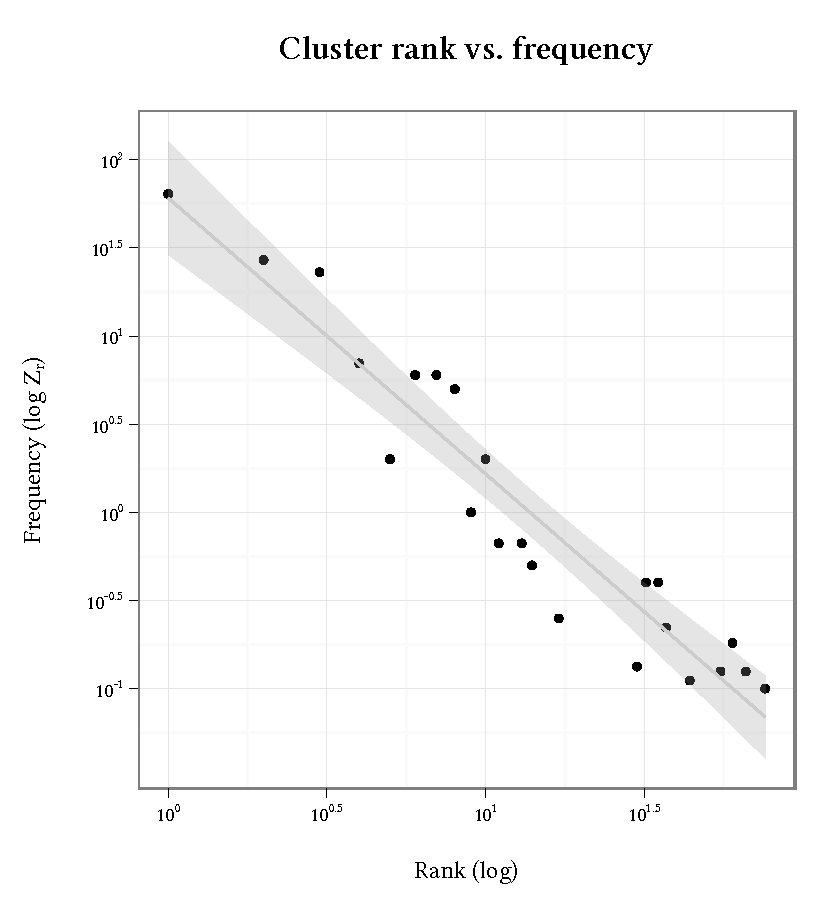
\includegraphics{cluster.pdf}
%\caption{Syllable contact clusters exhibit a log-log linear relationship between frequency and rank that is consistent with Zipf's Law.}
%\label{clus}
%\end{figure}
%
%Sparse distributions characterize the frequencies of many linguistic objects, from syntactic rules \citep{Yang2011b} to word \citep{Baroni2009} and phoneme \citep{Belevitch1956,Daland2011a} $n$-grams, but are also found in non-linguistic symbol systems \citep{Mandelbrot1954,Miller1957,Chomsky1958,Sproat2010} and randomly generated texts \citep{Miller1957,Li1992}. The importance of sparsity in this context is that it entails a long right tail, making it difficult to determine on statistical grounds alone which unobserved events are impossible and which are accidental gaps.
%
%\subsection{Good-Turing estimate}
%
%\citet{Good1953} proposes an estimate for the probability of all accidental gaps, $\hat{p}_0$, as the number of events that occur just once, $n_1$ divided by the number of observations.
%
%\begin{unlabeledexample}
%$\displaystyle \hat{p}_0 = \frac{n_1}{\displaystyle\sum N}$
%\end{unlabeledexample}
%
%\noindent In the CELEX data, $65$ clusters occur only once, and there are 873 cluster tokens, and thus $\hat{p}_0 = 0.074$. There is thus a non-trivial probability that many of the ``false positive'' clusters are in fact accidental gaps.
%
%\subsection{Sampling simulation}
%
%It is finally possible to ask what the lexicon might look like if it was stochastically generated from independent coda and onset frequencies, \emph{a la} \citeauthor{Pierrehumbert1994}, but also constrained by phonological neutralizations. The following method was repeated to generate a simulated lexicon.
%
%\begin{example}[Simulation procedure]
%\begin{tabular}{l l}
%a. & Sample a medial coda according to the observed probabilities  \\
%b. & Sample a medial onset according to the observed probabilities \\
%c. & Apply all matching \emph{SPE} rules to cluster formed by their concatenation \\
%\end{tabular}
%\end{example}
%
%The cluster frequencies for a single characteristic simulation are plotted in Figure \ref{sim}, along with observed frequencies; the two distributions are nearly indistinguishable. The sparse cluster inventory, previously taken as evidence for static constraints on syllable contact, is approximately what one would expect even if the only constraints on possible clusters are phonologically derived.
%
%\begin{figure}
%\centering
%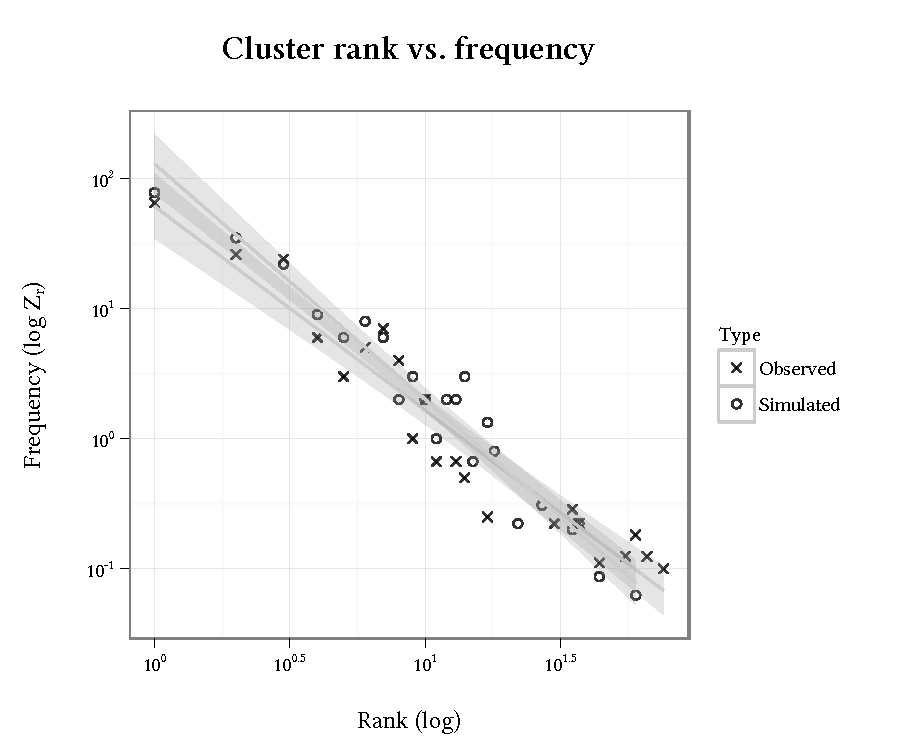
\includegraphics{sim.pdf}
%\caption{The observed cluster frequencies are closely matched by a simulated cluster inventory generated by random sampling, assuming independence and applying phonological neutralizations. The $Z_r$ transform \citep[][29]{Church1991} has been used to eliminate quantization in lower frequency bands.}
%\label{sim}
%\end{figure}
